\bfseries

\title[SIAM CS\&E 2011]{Reproducible Research: \\ Lessons from \\ the \textsc{Madagascar} Project}

\author[S. Fomel]{Sergey~Fomel}

\institute[UT Austin]
{
  Jackson School of Geosciences \\
  The University of Texas at Austin
}

\date{March 5, 2011}

\setbeamercolor{quotecol}{fg=black,bg=white}

\newcommand{\quotebox}[3]{
  \begin{beamercolorbox}[wd=\textwidth,center]{quotecol}
    \begin{quote}
      #1 
      \color{blue}{\emph{#2}, #3}
    \end{quote}
    \end{beamercolorbox}
}

\begin{frame}
  \MadLogo
%  \PTTCLogo
  \titlepage
\end{frame}

\section{Reproducible Research}

%\begin{frame}
%  \MadLogo
%  \frametitle{Outline}
%  \tableofcontents[pausesections]
%\end{frame}

\begin{frame}<beamer>
%  \MadLogo
  \frametitle{Outline}
  \tableofcontents[currentsection]
\end{frame}

\begin{frame}
%\MadLogo
\frametitle{What is Science?}

\begin{center}
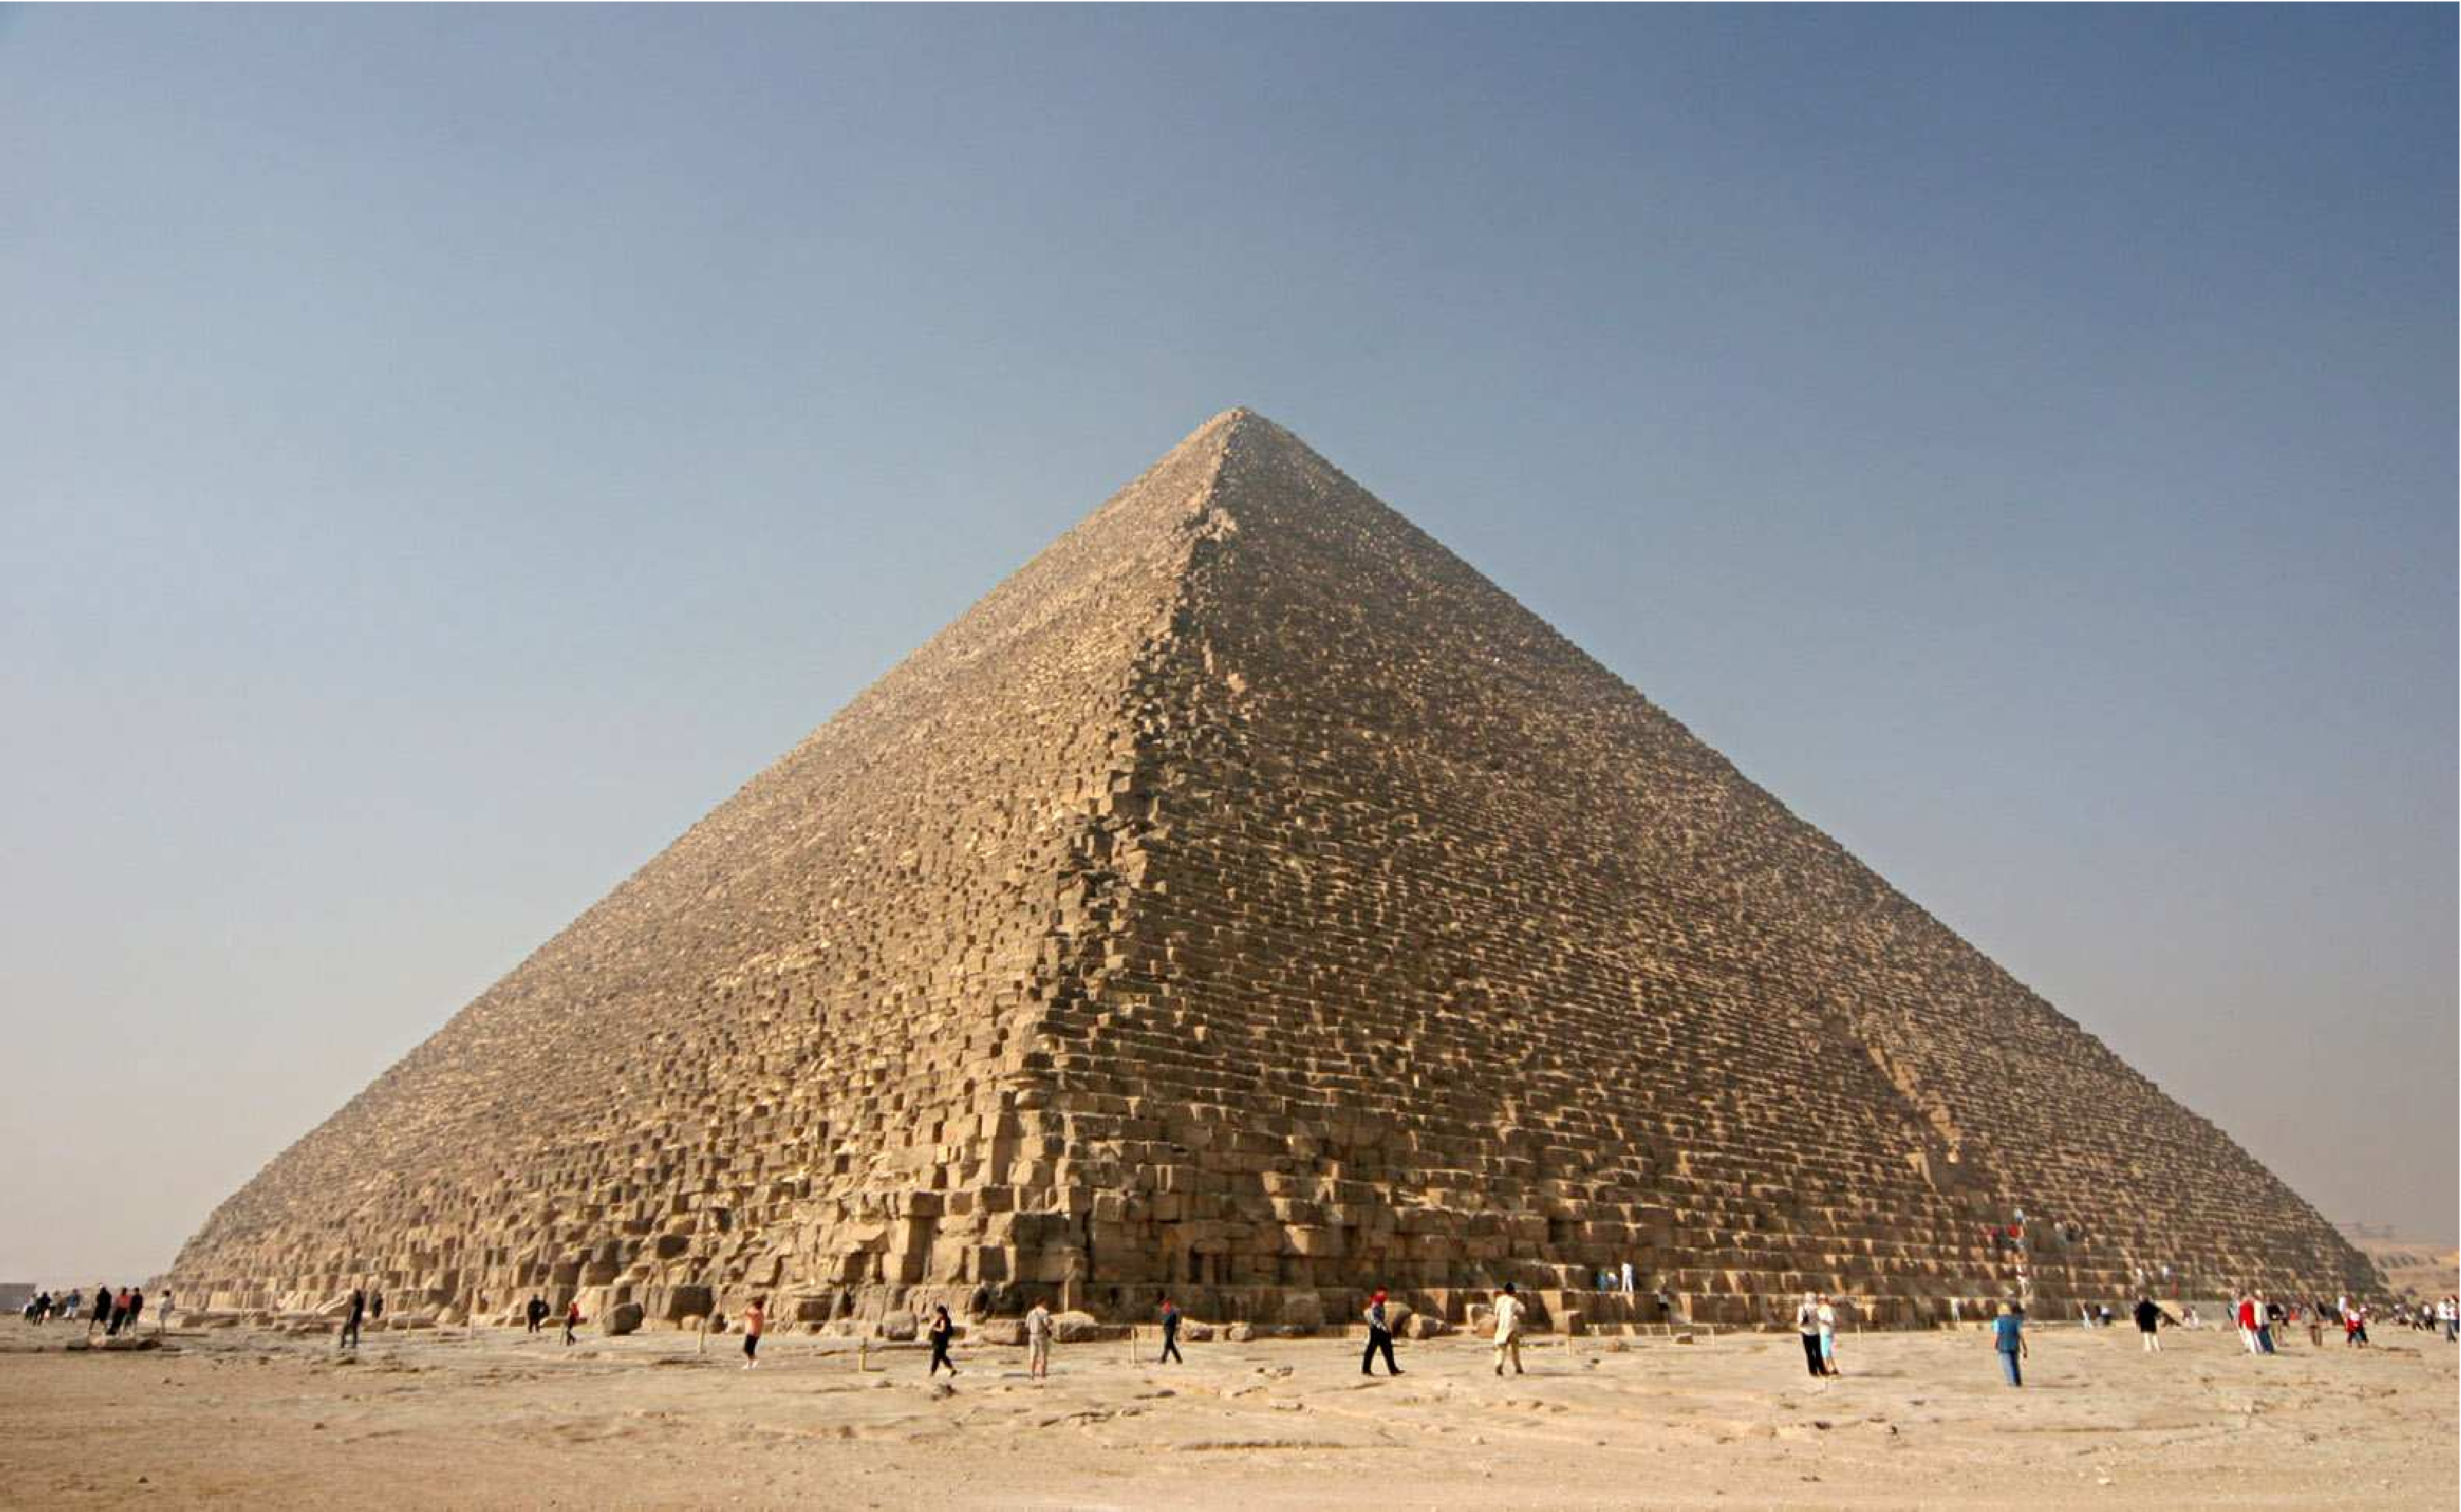
\includegraphics[height=0.8\textheight]{Fig/Kheops-Pyramid}
\end{center}
\end{frame}

\begin{frame}
%\MadLogo
\frametitle{What is Science?}

\quotebox{{\Large \color{blue}{Science}} is the systematic enterprise
  of gathering knowledge about the universe and organizing and
  condensing that knowledge into testable laws and theories. The
  success and credibility of science are anchored in the willingness
  of scientists to {\color{red}{independent testing and replication}}
  by other scientists. This requires the  {\color{red}{complete and
      open exchange of data, procedures and materials}}.}{\\ American
  Physical Society}{What is Science?}

\end{frame}

\begin{frame}
%\MadLogo
\frametitle{From Science to Open-Source Software}

\quotebox{{\Large \color{blue}{Abandoning the habit of secrecy}} in favor of process
  transparency and peer review was the crucial step by which alchemy
  became chemistry.  In the same way, it is beginning to appear that
  open-source development may signal the long-awaited maturation of
  software development as a discipline.}  {\\ Eric Raymond}{TAUP,
  2004}
\end{frame}

\begin{frame}
%\MadLogo
\frametitle{Communicating to a Skeptic}

\begin{center}

\includegraphics[height=0.85\textheight]{Fig/galileo}
\end{center}

\end{frame}

\begin{frame}
%\MadLogo
\frametitle{What is Reproducible Research?}

\begin{itemize}
\item Attaching software code and data to publications
\item Communicating computational results to a skeptic
\end{itemize}

\quotebox{An article about computational
    science in a scientific publication is not the scholarship itself,
    it is merely advertising of the scholarship. The actual
    scholarship is the complete software development environment and
    the complete set of instructions which generated the figures.}
  {J. Buckheit and D. Donoho}{WaveLab}

\end{frame}

\begin{frame}
 \frametitle{Reproducible Research Discussions}

  \begin{minipage}{0.3\textwidth}
  \begin{center}
  \framebox{
\includegraphics[width=\textwidth]{Fig/CiSE}}
  \vfill \ 
\end{center}
  \end{minipage} \hfill
   \begin{minipage}{0.65\textwidth}
  \begin{description}
    \item[ICASSP 2007] \ 
    \item[Berlin-6 2008] \
    \item[CiSE 2009] 
    \begin{itemize}
%    \item Fomel \& Claerbout
    \item Donoho et al.
    \item LeVeque
    \item Ping \& Eckel
    \item Stodden
    \end{itemize}
    \item[IEEE Signal Processing Magazine 2009] 
    \begin{itemize}
    \item Vandewalle et al.
     \end{itemize}
     \item[Yale Roundtable 2009] \
     \item[NSF Archive Workshop 2010] \ 
   \end{description}
  \end{minipage}

\vfill

\begin{itemize}
\item {\color{blue}{\textbf{\url{http://www.reproducibleresearch.net} }}}
\end{itemize}

\end{frame}

\begin{frame}
 \frametitle{Reproducible Research Discussions}

 \begin{description}
    \item[SIAM CS\&E 2011] \ 
    \begin{itemize}   
    \item Verifiable, Reproducible Research and Computational Science
%    \item J. Millman % (UC Berkeley)
%    \item {\color{blue}{\textbf{\url{http://meetings.siam.org/sess/dsp\_programsess.cfm?SESSIONCODE=11844}}}}
%    \item {\color{blue}{\textbf{\url{http://meetings.siam.org/sess/dsp\_programsess.cfm?SESSIONCODE=11845}}}}
    \end{itemize}
    \item[SIAM GS 2011] \
    \begin{itemize}   
    \item Reproducible Science and Open-Source Software in the Geosciences
%    \item B. Flemisch, K. Flornes, A. Rasmussen 
%    \item {\color{blue}{\textbf{\url{http://meetings.siam.org/sess/dsp\_programsess.cfm?SESSIONCODE=11822}}}}
%    \item {\color{blue}{\textbf{\url{http://meetings.siam.org/sess/dsp\_programsess.cfm?SESSIONCODE=11823}}}}
    \end{itemize}
    \item[AMP 2011] \
    \begin{itemize}   
    \item  Reproducible Research: Tools and Strategies for Scientific Computing
%    \item R. LeVeque, I. Mitchell, C. Moler, V. Stodden
    \item {\color{blue}{\textbf{\url{http://www.mitacs.ca/goto/amp\_reproducible}}}}
    \end{itemize}
    \item[ICIAM 2011] \
    \begin{itemize}
    \item Reproducible Research in Computational Science: What, Why and How
    \end{itemize}
    \end{description}
  \end{frame} 


\section{History of Madagascar}

\begin{frame}<beamer>
  \MadLogo
  \frametitle{Outline}
  \tableofcontents[currentsection]
\end{frame}

\begin{frame}
  \MadLogo
  \frametitle{Jon Claerbout's Story}

  {\flushright
  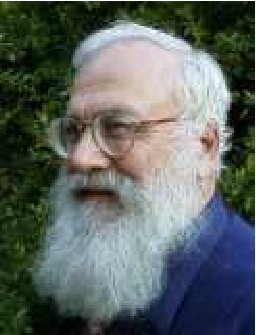
\includegraphics[height=0.2\textheight]{Fig/Claerbout}
  } 

  \begin{description}
  \item[1987] Sunview experience
  \begin{itemize}
  \item	Interactive programs are slavery
  \end{itemize}
  \item[1992] \LaTeX\ + \texttt{cake}
  \begin{itemize}
  \item Building books by a single command
  \end{itemize}
  \item[1990s] Ph.D. students
  \begin{itemize}
  \item \texttt{cake} to \texttt{make}, CD-Rom to WWW
  \end{itemize}
  \item[2001] Reproducible research paper in \emph{CiSE}
  \begin{itemize}
  \item {\color{blue}{The principal beneficiary is the author}}
  \end{itemize}
  \end{description}
\end{frame}

\begin{frame}
  \MadLogo
  \frametitle{Lesson 1}
{\flushright
  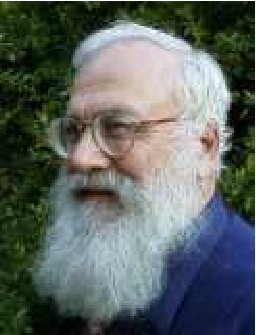
\includegraphics[height=0.2\textheight]{Fig/Claerbout}
  } 
\vfill
\begin{beamercolorbox}[wd=\textwidth,center]{quotecol}
\Large \color{blue}{\textbf{The principal beneficiary is the author.}}
\end{beamercolorbox}
\vfill

%  \begin{itemize}
%  \item The principal beneficiary is the author
%  \item Software code requires continuous maintenance
%  \item Maintenance requires an open community
%  \end{itemize}
\end{frame}

\begin{frame}
  \begin{center}
 
\includegraphics[height=0.5\textheight]{Fig/MadLogo} \\
 {\color{blue}{\textbf{\url{http://reproducibility.org/}}}} \\
 {\color{blue}{\textbf{\url{http://ahay.org/}}}} 
  \end{center}
\end{frame}

\begin{frame}
\MadLogo
  \frametitle{Ohloh.net about \textsc{Madagascar}}

\begin{minipage}{0.65\textwidth}
  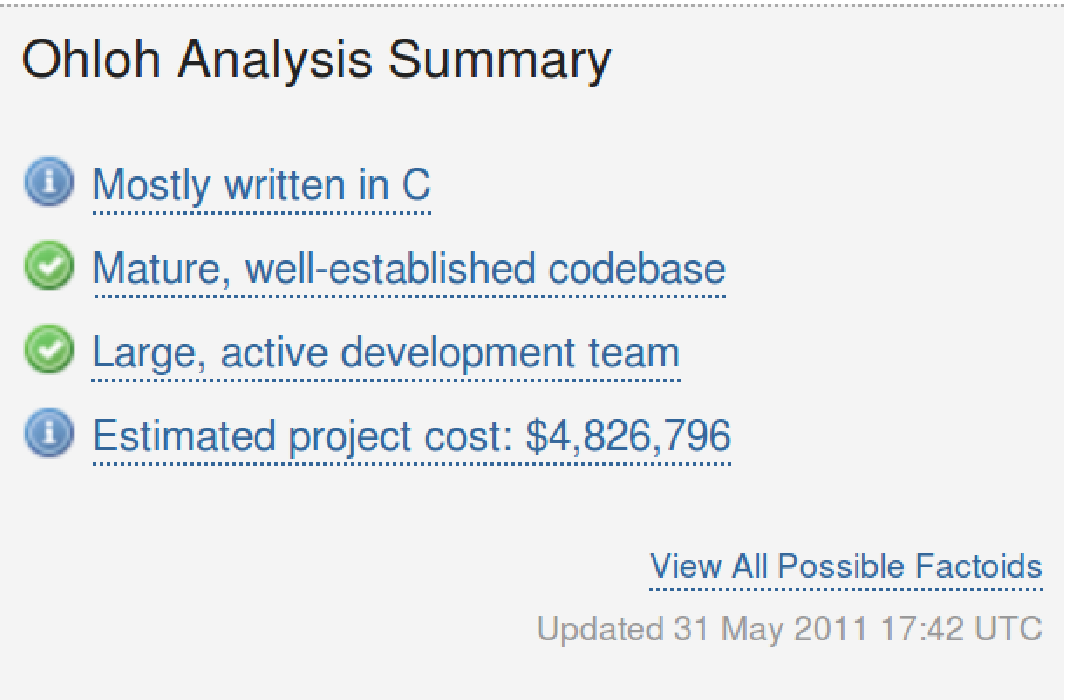
\includegraphics[height=0.3\textheight]{Fig/ohloh0} 
  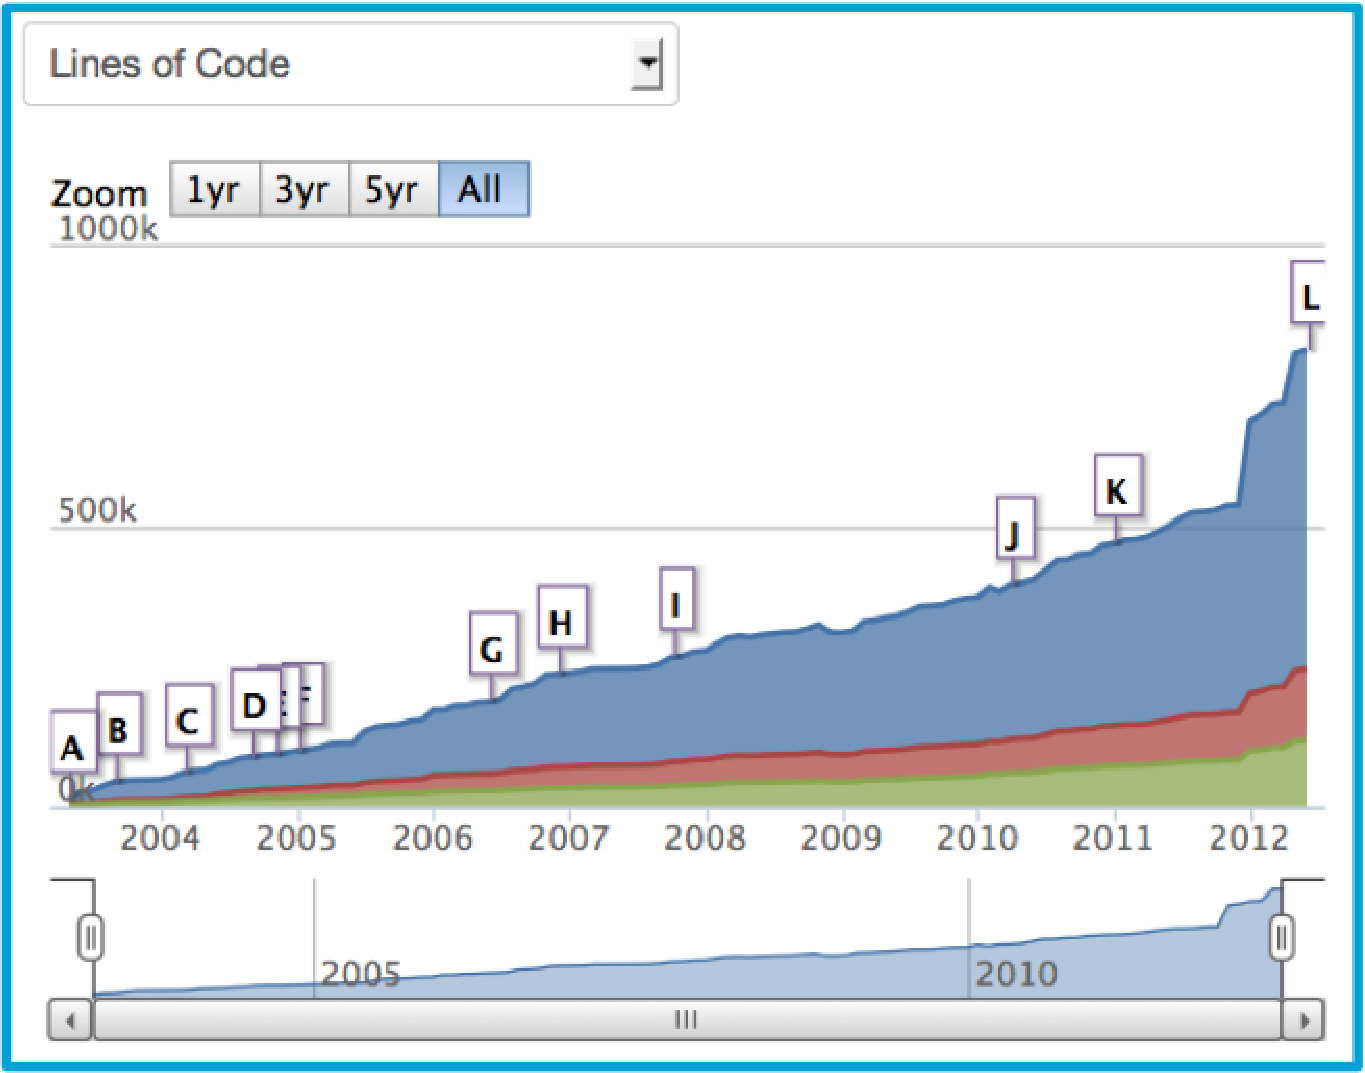
\includegraphics[width=\textwidth]{Fig/ohloh1}
\end{minipage}
\hfill
\begin{minipage}{0.3\textwidth}
  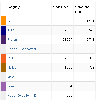
\includegraphics[width=\textwidth]{Fig/ohloh2}   
\end{minipage}

\end{frame}

\begin{frame}
  \MadLogo
  \frametitle{Lesson 2}

\begin{itemize}
\item {\color{blue}{\textbf{\url{http://www.ahay.org/wiki/Reproducible_Documents}}}}
\end{itemize}

\vfill
\begin{beamercolorbox}[wd=\textwidth,center]{quotecol}
\Large \color{blue}{\textbf{Each computation is a test.}}
\end{beamercolorbox}
\vfill


%  \begin{itemize}
%  \item The principal beneficiary is the author
%  \item Software code requires continuous maintenance
%  \item Maintenance requires an open community
%  \end{itemize}
\end{frame}


\begin{frame}
\MadLogo
\frametitle{Thanks}

\begin{itemize}
\item Tariq Alkhalifah, Vladimir Bashkardin, Jules Browaeys, \\
William Burnett, Cody Brown, Maria Cameron, \\
Lorenzo Casasanta, Joseph Dellinger, Jeff Godwin, \\
Gilles Hennenfent, Trevor Irons, Jim Jennings, Long Jin, \\
Roman Kazinnik, Siwei Li, Guochang Liu, Yang Liu, \\
Doug McCowan, Henryk Modzelewski, Colin Russell, \\
Paul Sava, Jeffrey Shragge, Xiaolei Song, \\
Eduardo Filpo Silva, Ioan Vlad, Jia Yan, Lexing Ying
\end{itemize}
\end{frame}


%\begin{frame}
%  \MadLogo
%  \frametitle{Access Geography}
%\begin{center}
%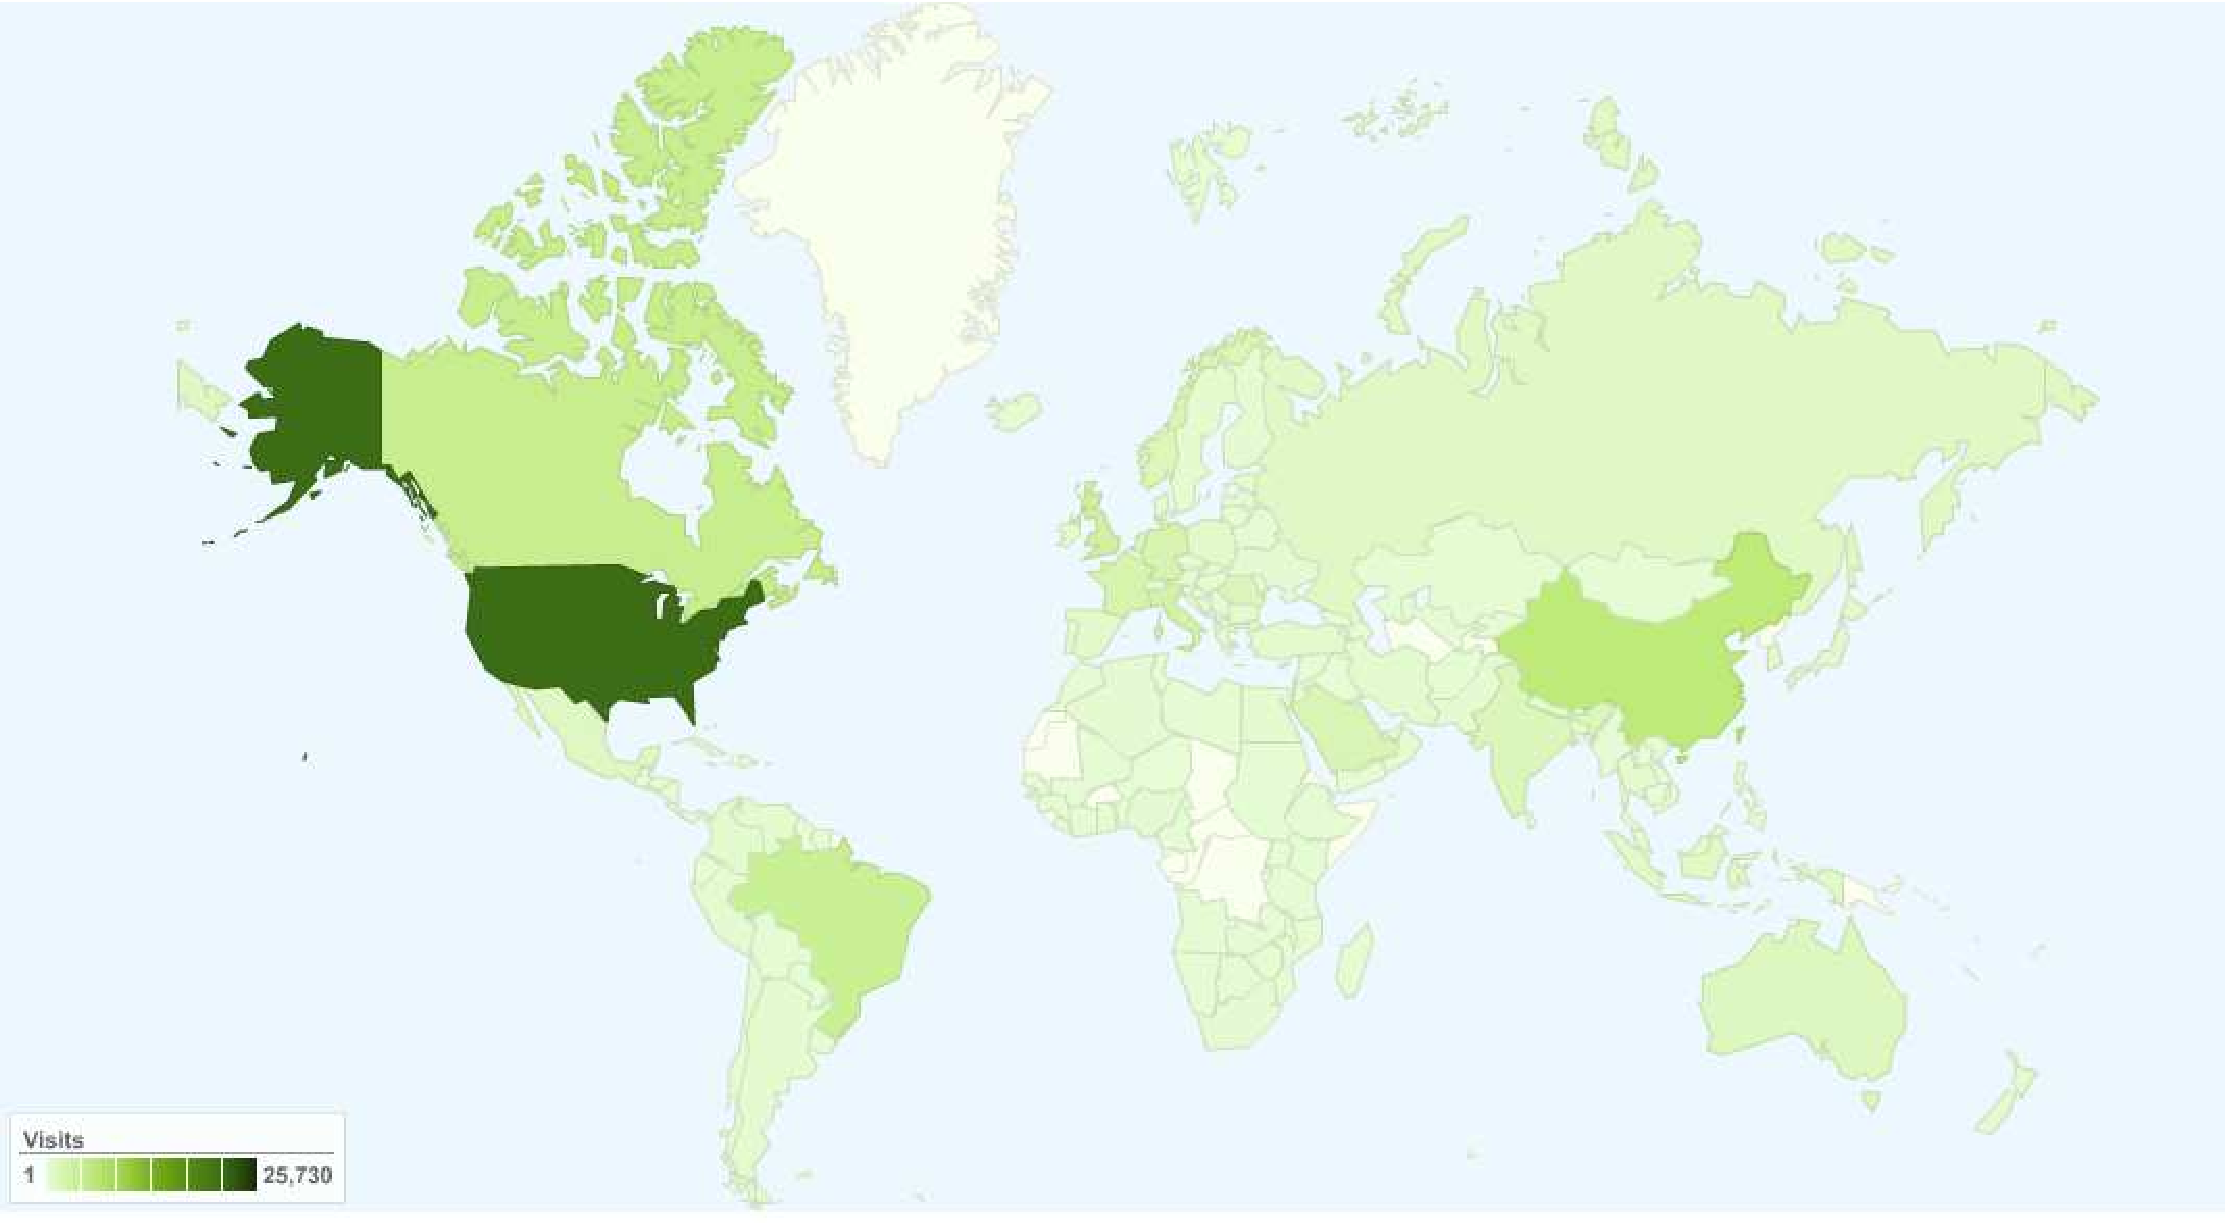
\includegraphics[width=0.85\textwidth]{Fig/map}  
%\end{center}
%\end{frame}

\begin{frame}
  \frametitle{School and Workshop: Vancouver 2006}
  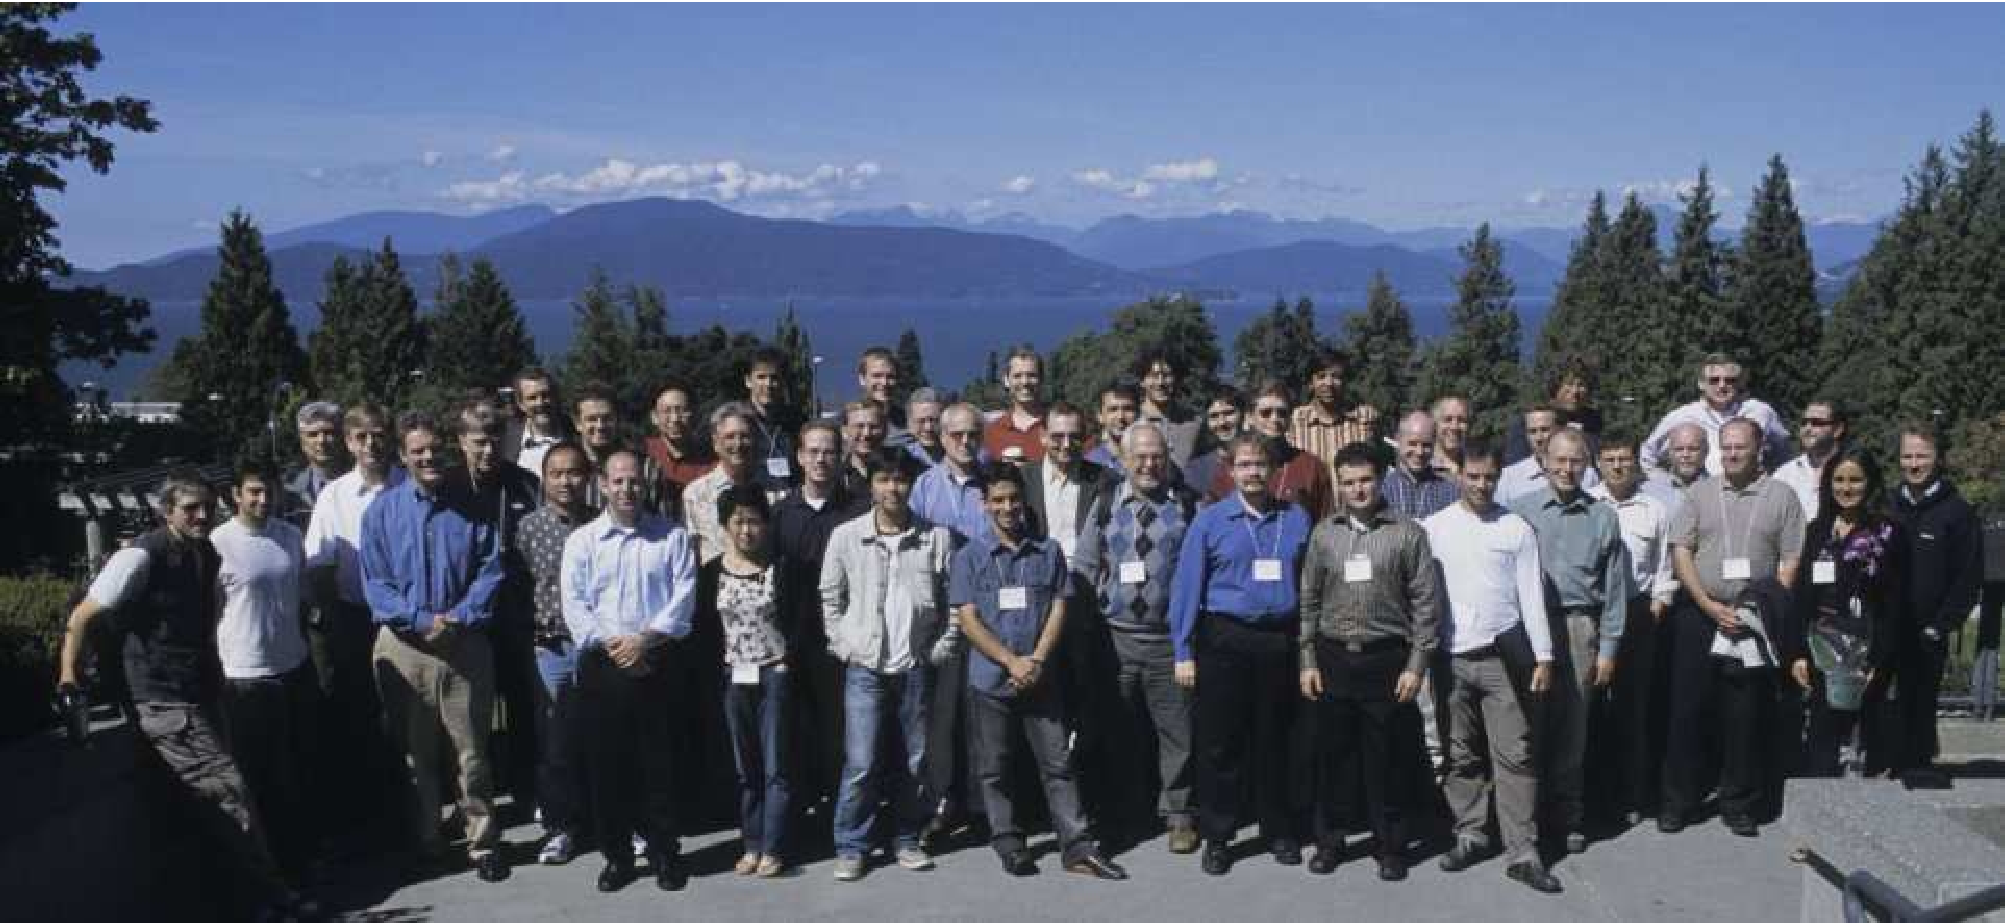
\includegraphics[width=\textwidth]{Fig/RSF2006}
\end{frame}

\begin{frame}
  \frametitle{School and  Workshop: Houston 2010}
  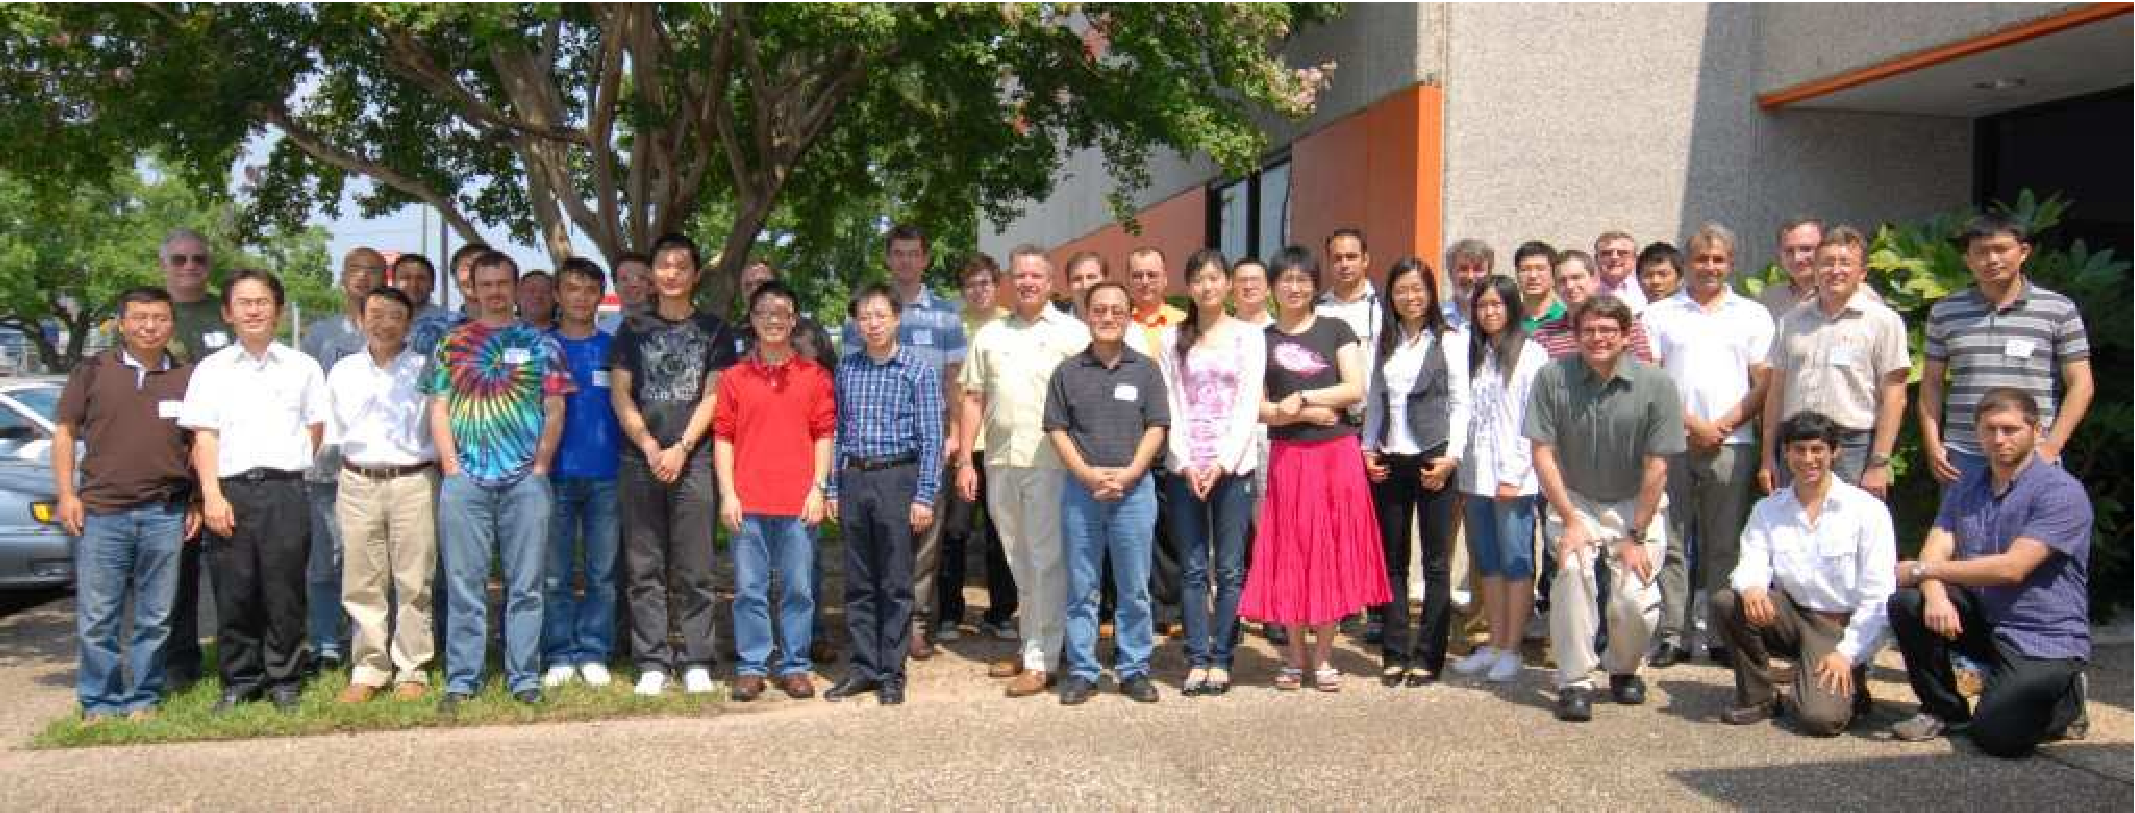
\includegraphics[width=\textwidth]{Fig/RSF2010}
\end{frame}

%\begin{frame}
%  \MadLogo
%\begin{center}
%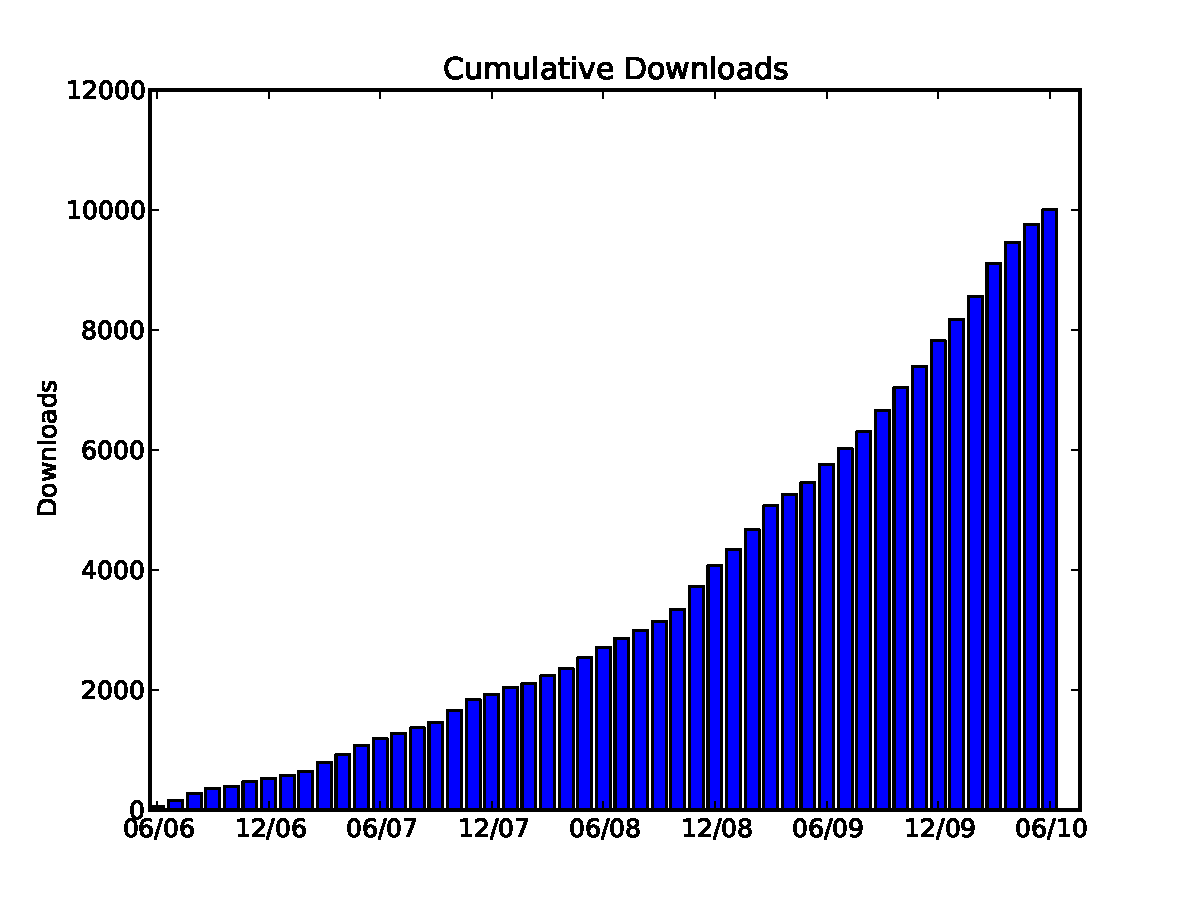
\includegraphics[height=\textheight]{Pylab/Fig/downloads}  
%\end{center}
%\end{frame}

\begin{frame}
  \MadLogo
  \frametitle{Lessons 3 and 4}

\vfill
\begin{beamercolorbox}[wd=\textwidth,center]{quotecol}
\Large \color{blue}{\textbf{Reproducibility requires maintenance.}}
\end{beamercolorbox}
\vfill
\begin{beamercolorbox}[wd=\textwidth,center]{quotecol}
\Large \color{blue}{\textbf{Maintenance requires an open community.}}
\end{beamercolorbox}
\begin{center}

\includegraphics[height=0.33\textheight]{Fig/books}
\end{center}

\end{frame}

\begin{frame}
  \MadLogo
  \frametitle{\textsc{Madagascar} Design}

\begin{minipage}{0.3\textwidth}
  \begin{center}
  \framebox{
\includegraphics[width=\textwidth]{Fig/unix}}
  \vfill \ 
\end{center}
  \end{minipage} \hfill
   \begin{minipage}{0.65\textwidth}
\begin{itemize}
  \item Multidimensional arrays as files
\end{itemize}
  \quotebox{Write programs that do one thing and do it well. Write
        programs to work together. Write programs to handle text
        streams, because that is a universal interface.}{\\ Doug McIlroy}{Unix}
  \end{minipage}
  
\end{frame}

\begin{frame}
\frametitle{\textsc{Madagascar} filter in C}
\MadLogo

\begin{code}[c]
\centering
\hfill
\begin{minipage}{0.9\textwidth}
\lstset{language=c,showstringspaces=false}
\lstinputlisting[frame=single]{clip.c}
\end{minipage}
\hfill
\end{code}

\end{frame}

\begin{frame}
\frametitle{\textsc{Madagascar} filter in Python}
\MadLogo

\begin{code}[python]
\centering
\hfill
\begin{minipage}{0.9\textwidth}
\lstinputlisting[frame=single]{clip.py}
\end{minipage}
\hfill
\end{code}

\end{frame}

\begin{frame}
\frametitle{\textsc{Madagascar} \texttt{SConstruct} script}
\MadLogo

\begin{code}[python]
\centering
\hfill
\begin{minipage}{0.9\textwidth}
\lstinputlisting[frame=single]{scons.py}
\end{minipage}
\hfill
\end{code}

\vfill

\begin{code}[bash]
\lstinputlisting[frame=none]{scons.sh}
\end{code}

\vfill

\begin{minipage}{0.65\textwidth}
\vfill
\begin{itemize}
\item  {\color{blue}{\textbf{\url{http://www.scons.org/}}}}
\end{itemize}
\end{minipage}
\begin{minipage}{0.25\textwidth}
\begin{center}

\includegraphics[height=0.1\textheight]{Fig/SCons}
\end{center}
\end{minipage}

\end{frame}

\begin{frame}
\MadLogo
%\frametitle{Reproducible Research Lessons}
\bfseries
\centering
  \begin{itemize}
  \item Reproducible research
    \begin{itemize}
    \item Attaching software and data to publications
    \item Computational experiments communicated to a skeptic
    \end{itemize}
  \item \textsc{Madagascar} Lessons
    \begin{enumerate}
    \item The principal beneficiary is the author.
    \item Each computation is a test.
    \item Reproducibility requires maintenance.
    \item Maintenance requires an open community.
    \end{enumerate}
\end{itemize}
    \begin{center}
      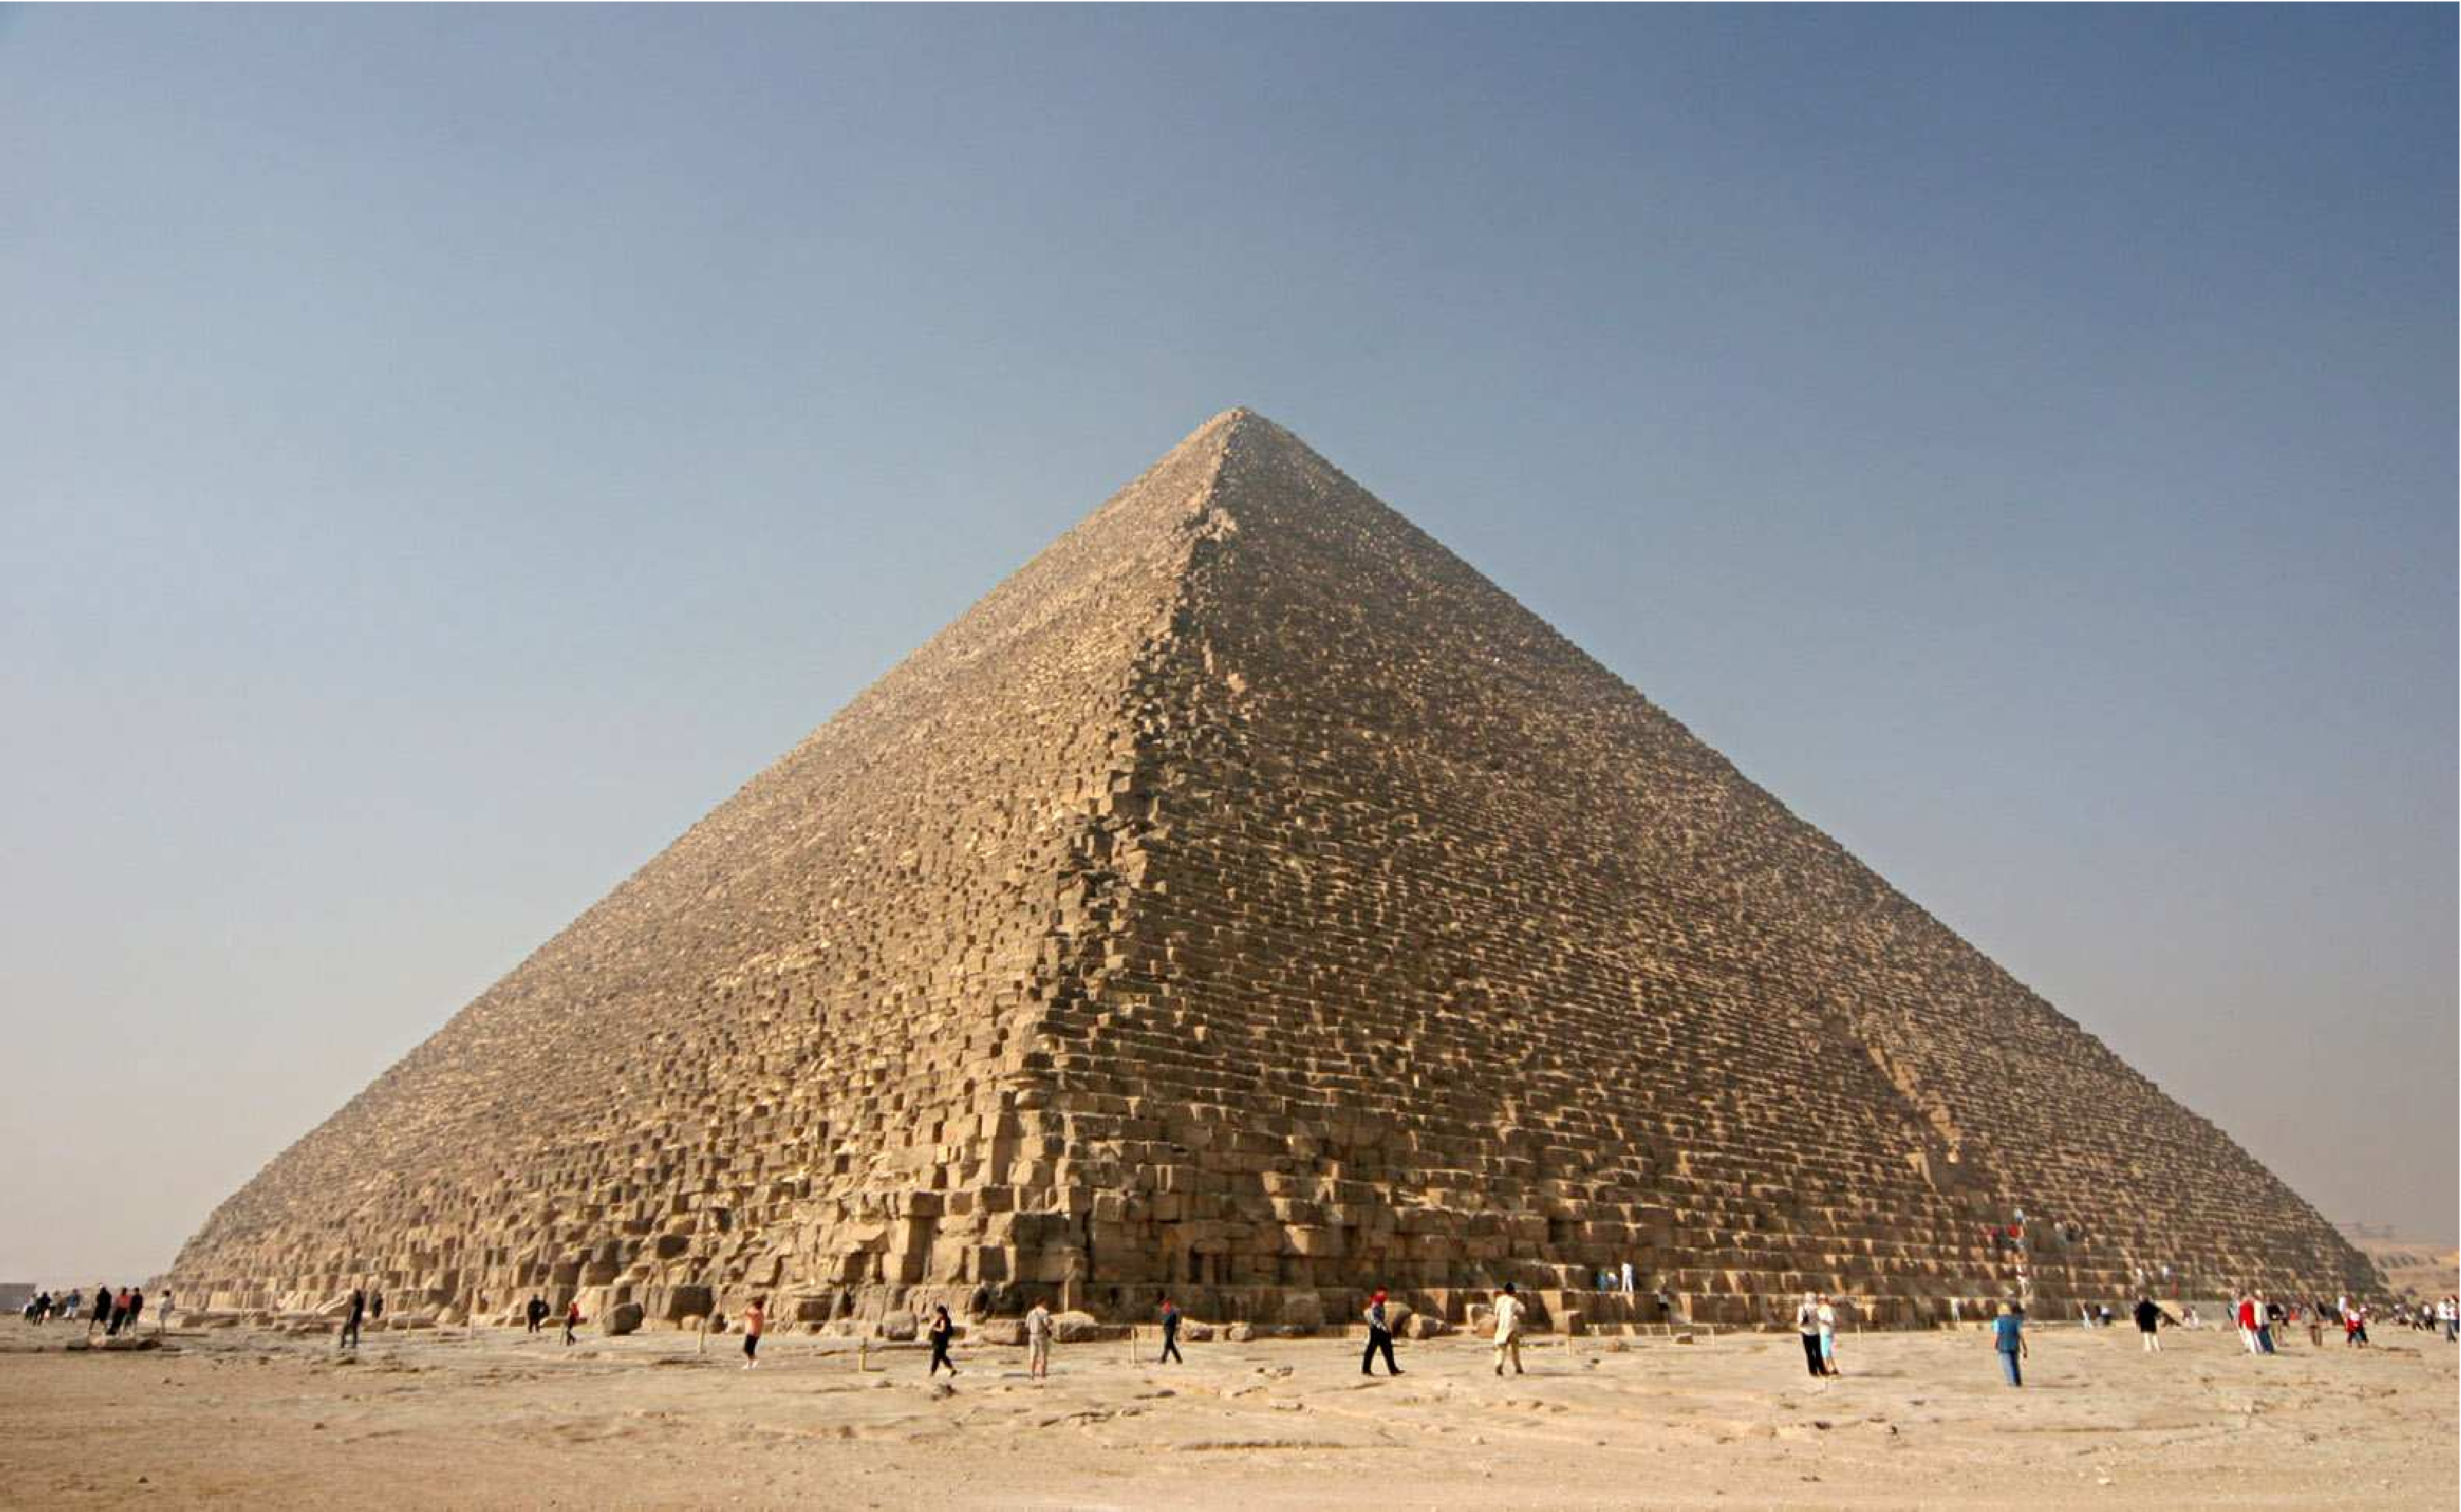
\includegraphics[height=0.4\textheight]{Fig/Kheops-Pyramid}
    \end{center}
  \end{frame}
